\chapter{Implementation and Evaluation}
\section{Training Mask R-CNN}
\noindent
	
	In this research, we take advantage of a pre-trained model of Mask R-CNN and fine-tune it to for our problem instead of training the whole architecture of Mask R-CNN from scratch due to the lack of time and resources. 
	
	Although Facebook's researchers published the official source code in 2018, we prefer using the unofficial one from Matterport Inc which was published in 2017 due to the majority of deep learning practitioner community (5k3 fork times compared to 9k6 ones, respectively). Further information, you can access the source code via this link \url{https://github.com/matterport/Mask_RCNN}.
	
	In addition, the whole training process was executed on Google's CoLab to take advantages of GPU power (which we did not have). Besides, the training loss and the validation loss, we also calculated mAP and mAR to evaluate the models more precisely.
	
\subsection{Configuration setting}
\noindent

	In the training phrase, focused on fine-tune several hyper-parameters that affected strongly for transfer learning technique. According to \cite{maskrcnn}, the default configuration was set based on Faster R-CNN due to its robustness on not only on detection task but also segmentation one. Look at Table \ref{table:hyperparameters} for more details about hyper-parameters.
	
	\begin{table}[H]
		\begin{tabularx}{1\textwidth} {
				| >{\raggedright\arraybackslash}X 
				| >{\raggedright\arraybackslash}X
				| >{\raggedright\arraybackslash}X 
				| >{\raggedright\arraybackslash}X
				| >{\raggedright\arraybackslash}X
				| >{\raggedright\arraybackslash}X
				| >{\raggedright\arraybackslash}X
				| >{\raggedright\arraybackslash}X
				| >{\raggedright\arraybackslash}X
				| >{\raggedright\arraybackslash}X
				| >{\raggedright\arraybackslash}X
				| >{\raggedright\arraybackslash}X
				| >{\raggedright\arraybackslash}X
				| >{\raggedright\arraybackslash}X  
				| >{\raggedright\arraybackslash}X | }
			\hline
			Model & Describe \\
			\hline
			IMAGE RESIZE MODE & Input image resizing. \\
			\hline
			STEPS PER EPOCH & Number of training steps per epoch. Don't set this too small to avoid spending a lot of time on validation stats. \\
			\hline
			VALIDATION STEPS & Number of validation steps to run at the end of every training epoch. A bigger number improves accuracy of validation stats, but slows down the training. \\
			\hline
			BACKBONE & Backbone network architecture. ResNet50 and ResNet101 are supported. \\
			\hline
			LEARNING RATE & Learning rate. \\
			\hline
			LEARNING MOMENTUM & Momentum \\
			\hline
			OPTIM & Optimization algorithm. \\
			\hline
			WEIGHT DECAY & Weight decay regularization. \\
			\hline
			LOSS WEIGHTS & Loss weights for more precise optimization. (Focus on desired loss) \\
			\hline
			
		\end{tabularx}
		\caption{Hyper-parameter description}
		\label{table:hyperparameters}
		
	\end{table}
	
	In Table \ref{table:hyperparameters}, we only list several hyper-parameters that are important in the fine-tune process. In addition, for more information of hyper-parameters, we recommend reader to read at \url{https://github.com/matterport/Mask_RCNN/blob/master/mrcnn/config.py}.
	
\subsection{Training}
\label{subsection:mrcnn_training}
\noindent

	As mentioned before, we used transfer learning technique to train Mask R-CNN. The dataset we used was described in Subsection \ref{subsection:dataset}. With a small pre-processing, we changed the annotation images and exported annotation's information (COCO's format) from it to fit Mask R-CNN's input requirement. In addition, we also applied data augmentation to increase the dataset size in order to avoid over-fitting problem. To be more precise, we created more images by:
	
	\begin{itemize}
		\item Flipping 50\% images vertically and horizontally, respectively.
		\item Rotating all images by 90, 180, and 270 degree.
		\item Multiplying images by a random value sampled uniformly from the interval [0.8, 1.5], making some images darker and others brighter.
		\item Blurring images using a gaussian kernel with a random standard deviation sampled uniformly (per image) from the interval [0.0, 5.0].
	\end{itemize}
	
	In the training process, we took advantages by using a pre-trained of Mask R-CNN trained on COCO dataset. Because we only trained the head of the network, we decided to use 20-30 epochs.
	
	\textbf{Noted:} Mask RCNN includes a FCN \cite{fcn} and Faster RCNN \cite{f}. Hence, loss weight includes RPN (class loss, bbox loss) and Mask RCNN (class loss, bbox loss, and mask loss).
	
	The result is illustrated in Table \ref{table:exp1} and \ref{table:exp2}. All of these configurations were set and fin-tuned based on \cite{maskrcnn} and \url{https://github.com/matterport/Mask_RCNN}.
	

	\begin{longtable}[c]{|p{0.2\textwidth}|p{0.14\textwidth}|p{0.14\textwidth}|p{0.14\textwidth}|p{0.14\textwidth}|}
		\hline
		& \multicolumn{1}{c|}{\textbf{Test 1}} & \multicolumn{1}{c|}{\textbf{Test 2}} & \multicolumn{1}{c|}{\textbf{Test 3}} & \multicolumn{1}{c|}{\textbf{Test 4}} \\ \hline
		\endfirsthead
		%
		\multicolumn{5}{c}%
		{{\bfseries Table \thetable\ continued from previous page}}
		\endhead
		%
		\textbf{Backbone} & Resnet50 & Resnet50 & Resnet101 & Resnet101 \\ \hline
		\textbf{Optimizer} & SGD & Adam & SGD & Adam \\ \hline
		\textbf{Learning rate} & 0.001 & 0.001 & 0.001 & 0.001 \\ \hline
		\textbf{Weight decay} & 0.0005 & 0.0005 & 0.0005 & 0.0005 \\ \hline
		\textbf{Momentum} & 0.9 & 0.9 & 0.9 & 0.9 \\ \hline
		\textbf{Epoch} & 20 & 20 & 20 & 20 \\ \hline
		\textbf{Train - Val step} & 150 - 50 & 150 - 50 & 150 - 50 & 150 - 50 \\ \hline
		\textbf{Detection min confidence} & 0 & 0 & 0.9 & 0.9 \\ \hline
		\textbf{Detection NMS threshold} & 0.9 & 0.9 & 0.9 & 0.9 \\ \hline
		\textbf{RPN anchor scale} & 16, 32, 64, 128, 256 & 16, 32, 64, 128, 256 & 16, 32, 64, 128, 256 & 16, 32, 64, 128, 256 \\ \hline
		\textbf{Resize mode} & square & square & square & square \\ \hline
		\multirow{6}{*}{\textbf{Loss weight}} & rpn class loss: 1.0, & rpn class loss: 1.0, & rpn class loss: 1.0, & rpn class loss: 1.0, \\ \cline{2-5} 
		& rpn bbox loss: 1.0, & rpn bbox loss: 1.0, & rpn bbox loss: 1.0, & rpn bbox loss: 1.0, \\ \cline{2-5} 
		& mrcnn class loss: 1.0, & mrcnn class loss: 1.0, & mrcnn class loss: 1.0, & mrcnn class loss: 1.0, \\ \cline{2-5} 
		
		& mrcnn bbox loss: 1.0, & mrcnn bbox loss: 1.0, & mrcnn bbox loss: 1.0, & mrcnn bbox loss: 1.0, \\ \cline{2-5} 
		
		& mrcnn mask loss: 3.0 & mrcnn mask loss: 3.0 & mrcnn mask loss: 3.0 & mrcnn mask loss: 3.0 \\ \hline
		
		\textbf{mAP} & 0.511111 & 0.822222222 & 0.977777777 & 0.0 \\ \hline
		\textbf{mAR} & 0.533333 & 0.837037037 & 0.977777777 & 0.0 \\ \hline
%		\textbf{NOTE} & loss weight balance helps improving the result & Adam shows better much results but training time is slower than SGD & SGD shows it is better in using resnet101 & Training loss went NaN value because lr is high &  \\ \hline
%		
		\caption{Experiment results}
		\label{table:exp1}
	\end{longtable}

	
	% Please add the following required packages to your document preamble:
	% \usepackage{multirow}
	% \usepackage{longtable}
	% Note: It may be necessary to compile the document several times to get a multi-page table to line up properly
	\begin{longtable}[c]{|p{0.2\textwidth}|p{0.13\textwidth}|p{0.13\textwidth}|p{0.13\textwidth}|p{0.13\textwidth}|}
		\hline
		& \multicolumn{1}{c|}{\textbf{Test 5}} & \multicolumn{1}{c|}{\textbf{Test 6}} & \multicolumn{1}{c|}{\textbf{Test 7}} & \multicolumn{1}{c|}{\textbf{Test 8}} \\ \hline
		\endhead
		%
		\textbf{Backbone} & Resnet101 & Resnet101 & Resnet50 & Resnet101 \\ \hline
		\textbf{Optimizer} & Adam & SGD & SGD & SGD \\ \hline
		\textbf{Learning rate} & 0.0001 & 0.0001 & 0.001 & 0.001 \\ \hline
		\textbf{Weight decay} & 0.0005 & 0.0005 & 0.0005 & 0.0005 \\ \hline
		\textbf{Momentum} & 0.9 & 0.9 & 0.7 & 0.7 \\ \hline
		\textbf{Epoch} & 30 & 30 & 30 & 30 \\ \hline
		\textbf{Train - Val step} & 150 - 50 & 150-50 & 150 - 50 & 150 - 50 \\ \hline
		\textbf{Detection min confidence} & 0.9 & 0.9 & 0.7 & 0.7 \\ \hline
		\textbf{Detection NMS threshold} & 0.9 & 0.9 & 0.7 & 0.7 \\ \hline
		\textbf{RPN anchor scale} & 16, 32, 64, 128, 256 & 16, 32, 64, 128, 256 & 16, 32, 64, 128, 256 & 16, 32, 64, 128, 256 \\ \hline
		\textbf{Resize mode} & square & square & square & square \\ \hline
		
		\multirow{5}{*}{\textbf{Loss weight}} & rpn class loss: 1.0, & rpn class loss: 1.0, & rpn class loss: 1.0, & rpn class loss: 1.0, \\ \cline{2-5} 
		& rpn bbox loss: 1.0, & rpn bbox loss: 1.0, & rpn bbox loss: 1.0, & rpn bbox loss: 1.0, \\ \cline{2-5} 
		& mrcnn class loss: 1.0, & mrcnn class loss: 1.0, & mrcnn class loss: 1.0, & mrcnn class loss: 1.0 \\ \cline{2-5} 
		& mrcnn bbox loss: 1.0, & mrcnn bbox loss: 1.0, & mrcnn bbox loss: 1.0, & mrcnn bbox loss: 1.0, \\ \cline{2-5} 
		& mrcnn mask loss: 3.0 & mrcnn mask loss: 3.0 & mrcnn mask loss: 3.0 & mrcnn mask loss: 3.0 \\ \hline
		
		\textbf{mAP} & 0.9629629629 & 0.9419753 & 0.16296298 & 0.9407408 \\ \hline
		\textbf{mAR} & 0.9703703703 & 0.9703703 & 0.16296298 & 0.9851852 \\ \hline
%		\textbf{NOTE} & ??? & ??? & SGD not works well with resnet50 &  \\ \hline
	
	\caption{Experiment results}
	\label{table:exp2}
	\end{longtable}
	
	Firstly, we started our training process with \textit{Test 1} and \textit{Test 2} in order to find out which optimizer was better than the other. In general, it is noticeable that Adam optimizer converged slightly faster than SGD one. Moreover, model with Adam optimizer showed a much better mAP and mAR compared to model with SGD. Yet, the total loss, especially the mask loss was still high (more than 0.4 and 0.2, respectively). Let's look at Figure \ref{fig:loss_12} and \ref{fig:mask_loss_12} for more details.
	
	\begin{figure}[H]
		\centering
		\subcaptionbox{Total loss in Test 1.}{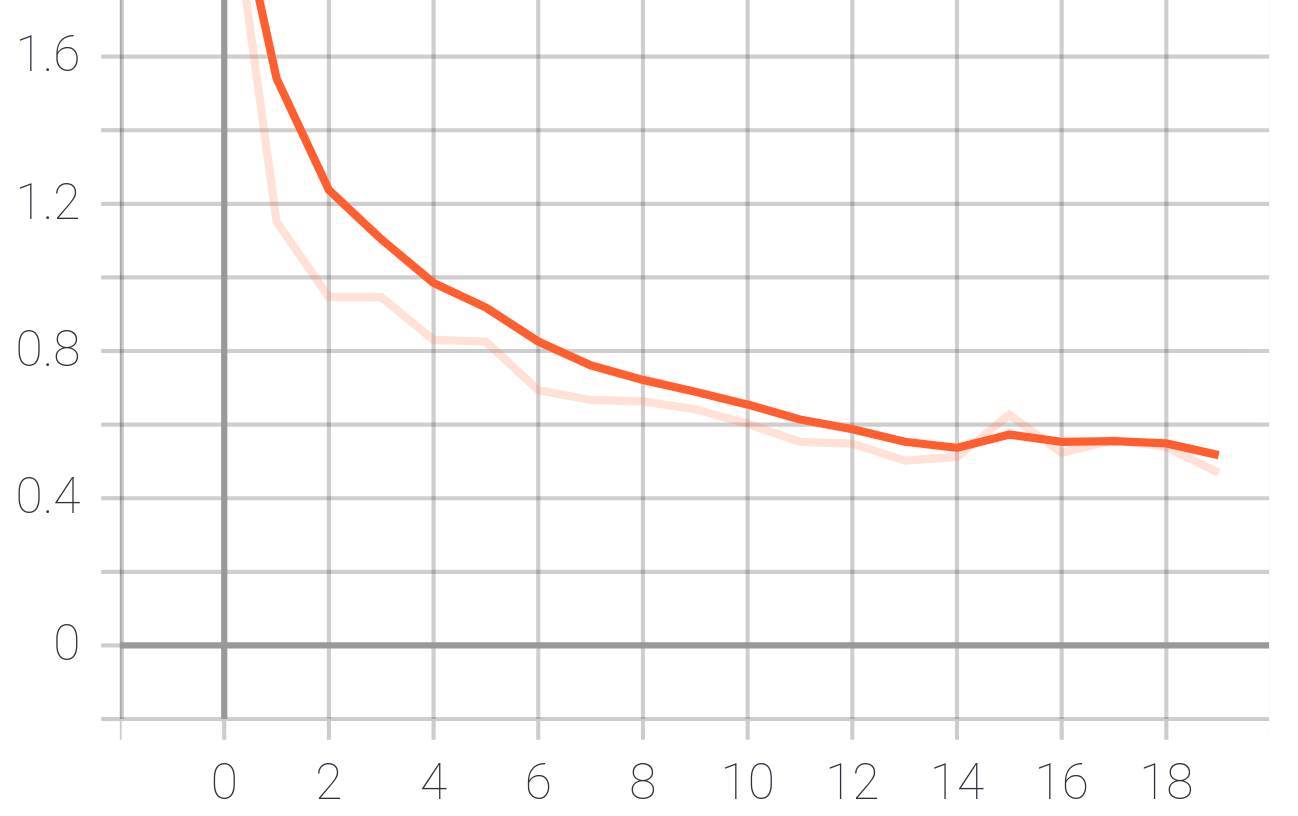
\includegraphics[width=0.45\textwidth]{./hinhanh/chap6/loss_t1.png}}%
		\hfill % <-- Seperation
		\subcaptionbox{Total loss in Test 2.}{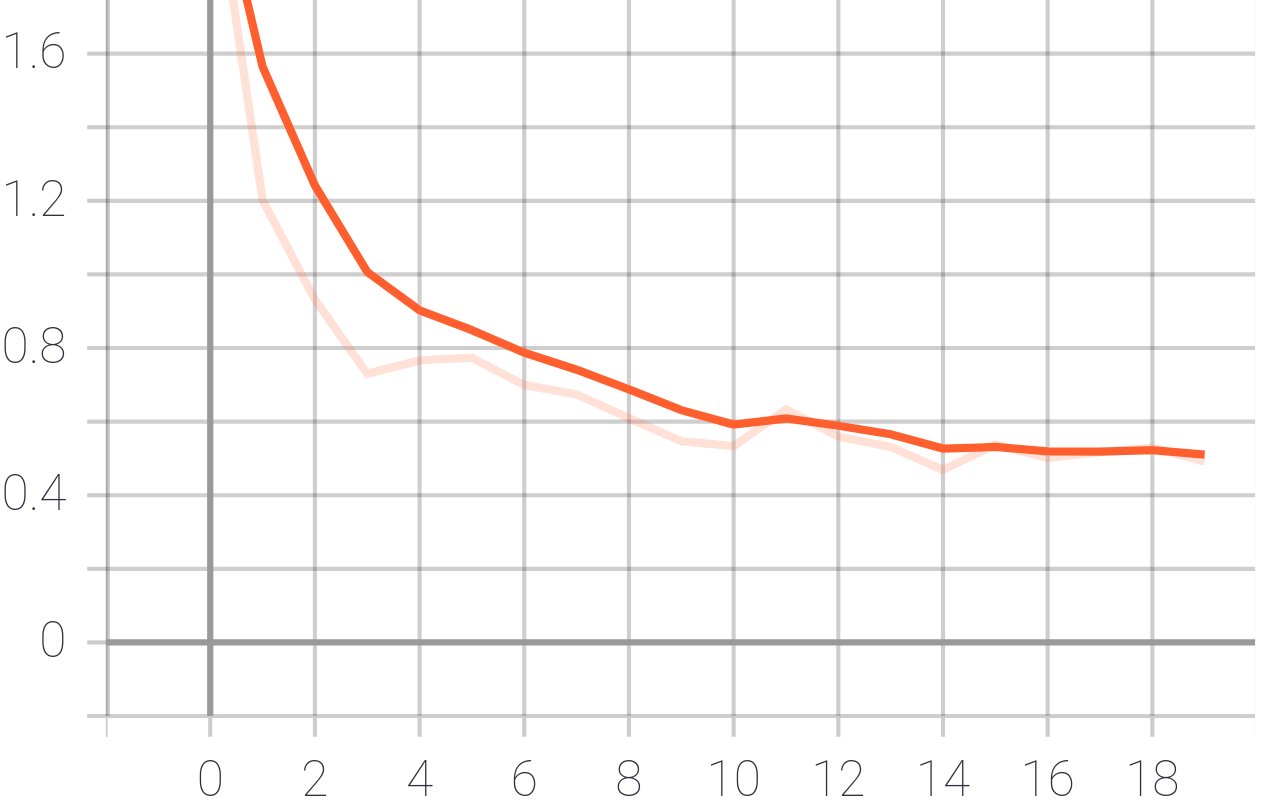
\includegraphics[width=0.45\textwidth]{./hinhanh/chap6/loss_t2.png}}%
		\hfill % <-- Seperation
		\caption{Comparison between Test 1 and Test 2 training loss.}
		\label{fig:loss_12}
	\end{figure}
	
	\begin{figure}[H]
		\centering
		\subcaptionbox{Mask loss in Test 1.}{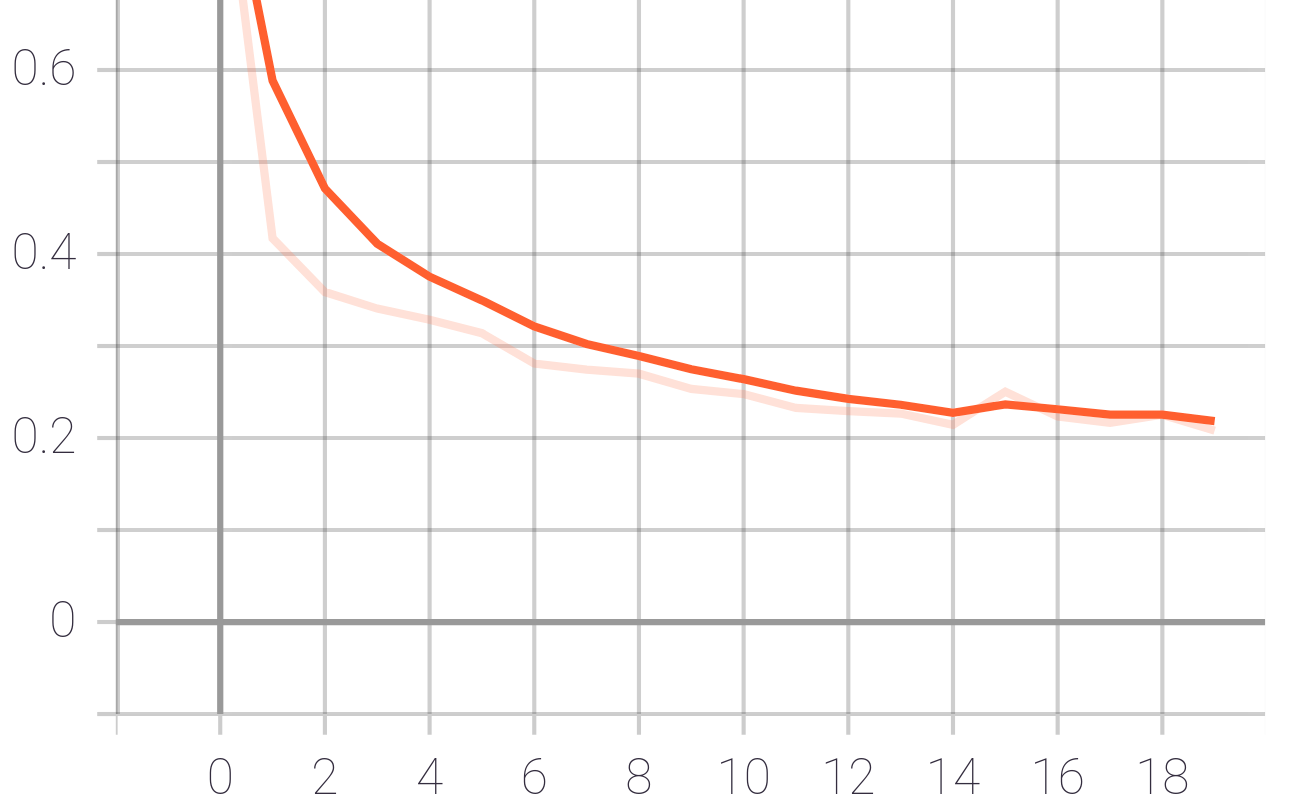
\includegraphics[width=0.45\textwidth]{./hinhanh/chap6/mask_loss_t1.png}}%
		\hfill % <-- Seperation
		\subcaptionbox{Mask loss in Test 2.}{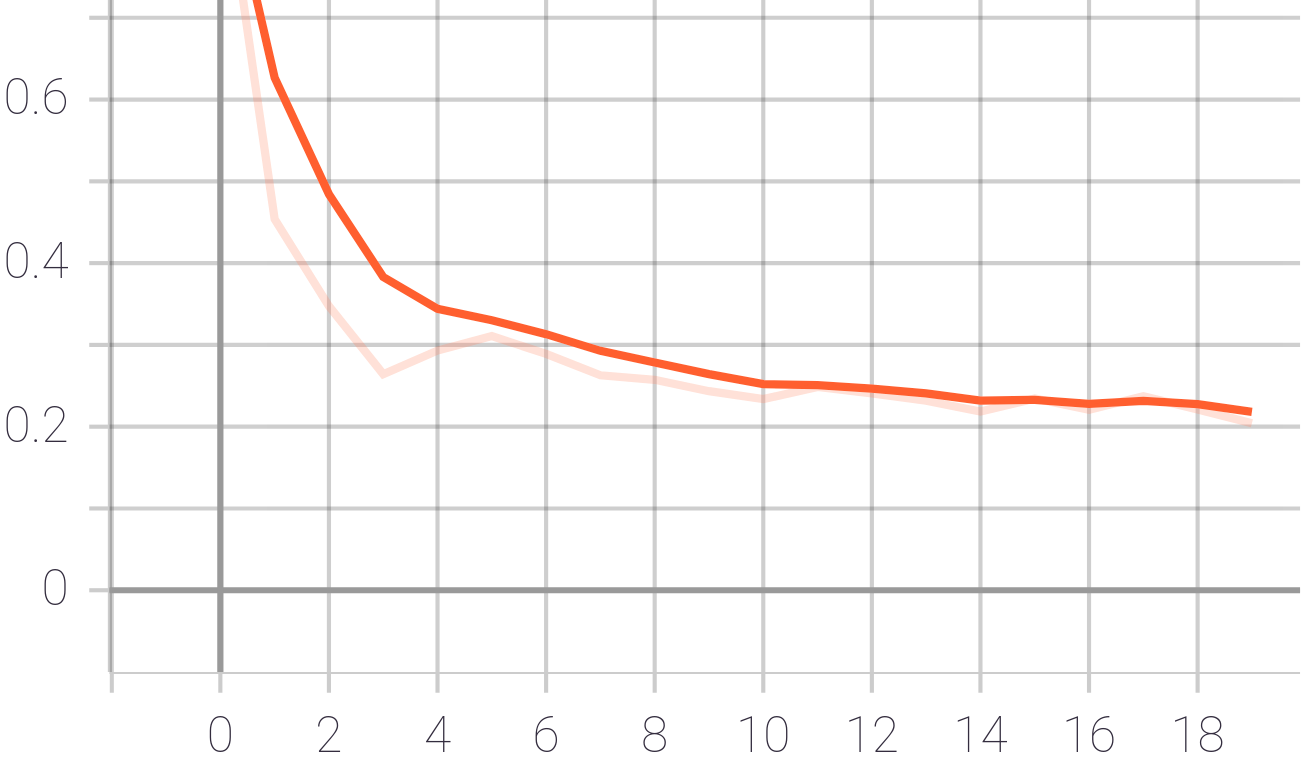
\includegraphics[width=0.45\textwidth]{./hinhanh/chap6/mask_loss_t2.png}}%
		\hfill % <-- Seperation
		\caption{Comparison between Test 1 and Test 2 training mask loss.}
		\label{fig:mask_loss_12}
	\end{figure}

\noindent	
	\textbf{Noted:} In training phrase, we mostly paid attention for the mask loss due to the characteristic of the problem which was instance segmentation. herefore, we altered the weight balance with the ratio was 1.0-1.0-1.0-1.0-3.0 in order to calculate the circumference of HC with the minimum error using the generated mask.
	
 	In next the experiments, we changed the backbone from ResNet50 to ResNet101 to see could we actually improve the model by going deeper? Besides, we also adjust the detection minimum confidence from 0 to 0.9 (we set it as 0 only the test the pre-trained at first). Hence, the results were remarkably significant. In \textit{Test 3}, with ResNet101, we improved the model mAP and mAR scores from ~0.5 to 0.97777 which were the highest scores in lots of experiments we had proceeded. 
 	
 	However, in \textit{Test 4} we replaced SGD by Adam again to check which one was better with ResNet101. Thus, the total loss of \textit{Test 4} unexpectedly went to NaN. Naturally, we had a hypothesis was that Adam optimizer was sensitive to the high learning rate (overshooting problem). Therefore, in \textit{Test 5} we decreased the learning rate to 0.0001, consequently, we could boost mAP and mAR score to 0.9419753 and 0.9703703, respectively. So the hypothesis was proved, it was due to the high learning rate that caused overshooting problem to \textit{Test 4}.
 	
	Although, Adam optimizer with ResNet50/Resnet101 backbone also showed a remarkable result \textit{Test 5}, SGD optimizer with ResNet101 backbone illustrated the improvement in results of \textit{Test 3} and \textit{Test 8} with mAP and mAR are (0.977777, 0.977777) and (0.9407408, 0.9851852), respectively. Moreover, based on \textit{Test 1} and \textit{Test 7}, it was confirmed that SGD did not work well with ResNet50.
	
	\begin{figure}[H]
		\centering
		\subcaptionbox{Total loss in Test 3.}{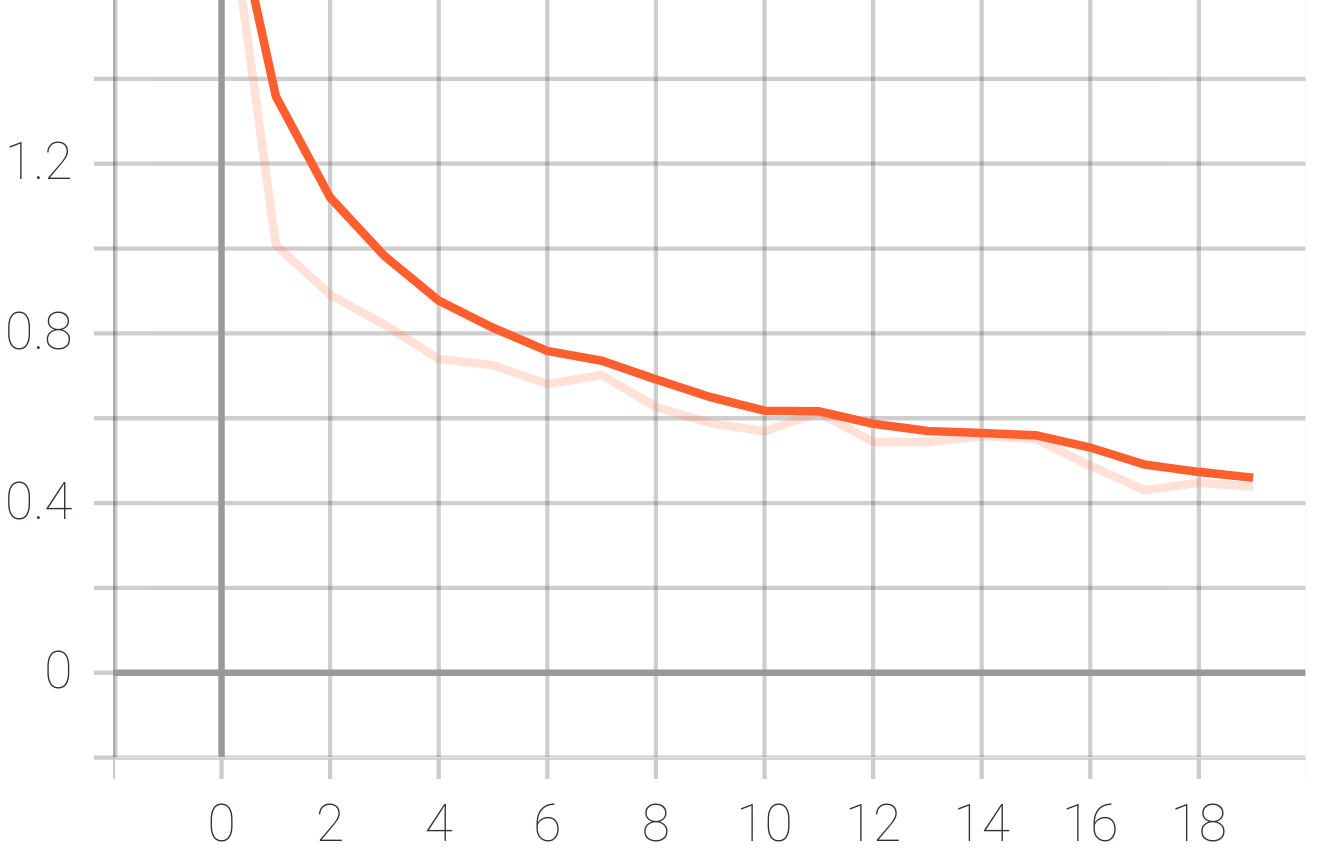
\includegraphics[width=0.45\textwidth]{./hinhanh/chap6/loss_t3.png}}%
		\hfill % <-- Seperation
		\subcaptionbox{Total loss in Test 10.}{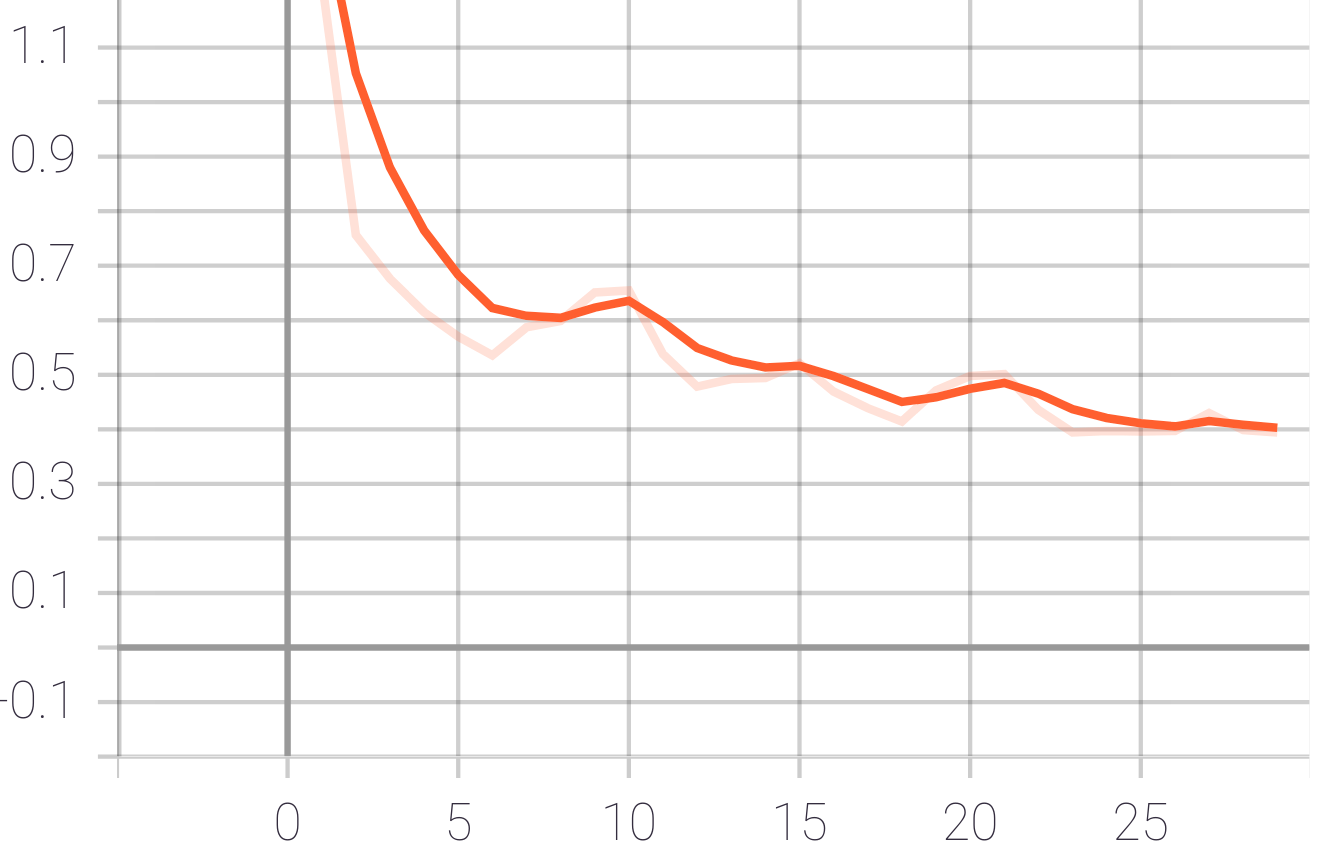
\includegraphics[width=0.45\textwidth]{./hinhanh/chap6/loss_t10.png}}%
		\hfill % <-- Seperation
		\caption{Comparison between Test 3 and Test 10 training loss.}
		\label{fig:loss_12}
	\end{figure}
	
	\begin{figure}[H]
		\centering
		\subcaptionbox{Mask loss in Test 3.}{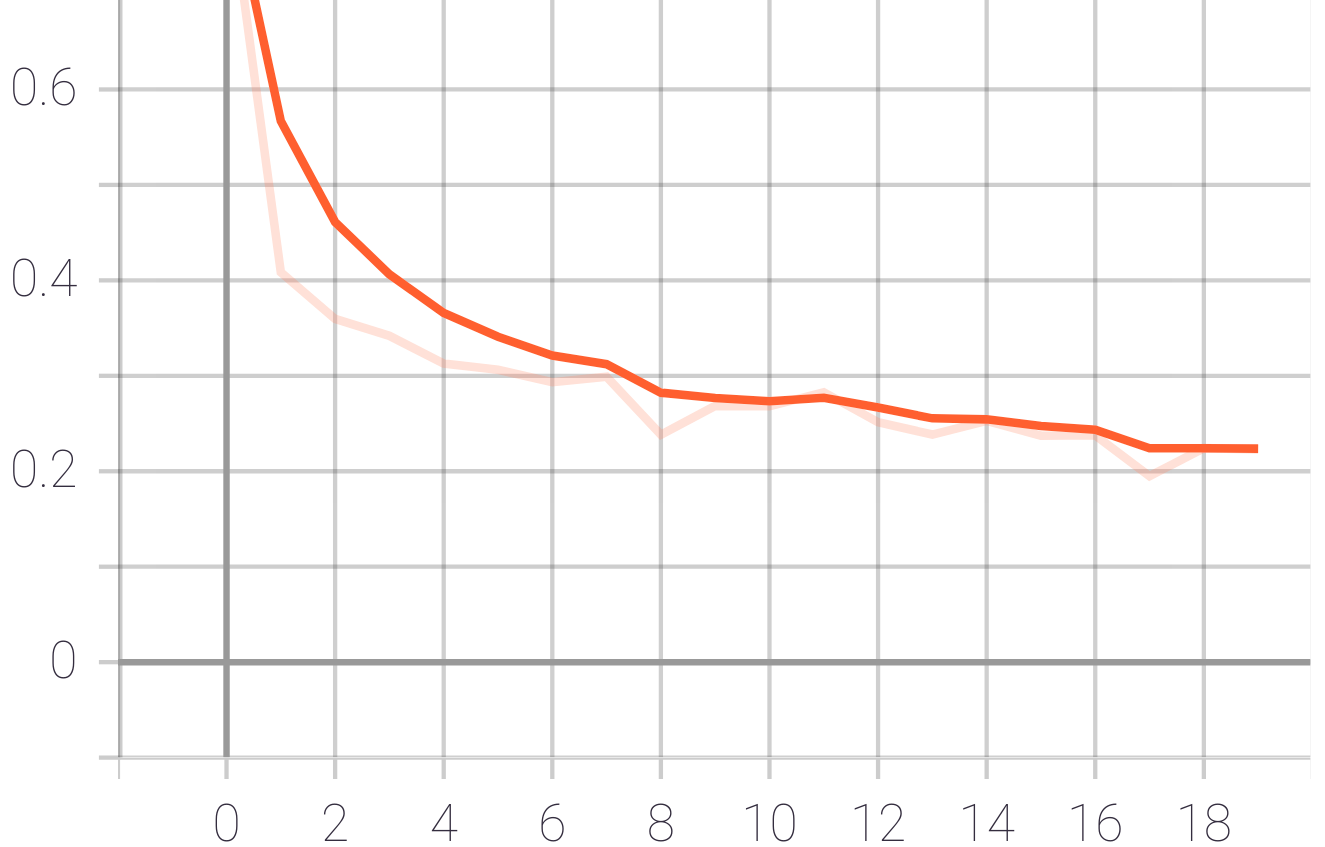
\includegraphics[width=0.45\textwidth]{./hinhanh/chap6/mask_loss_t3.png}}%
		\hfill % <-- Seperation
		\subcaptionbox{Mask loss in Test 10.}{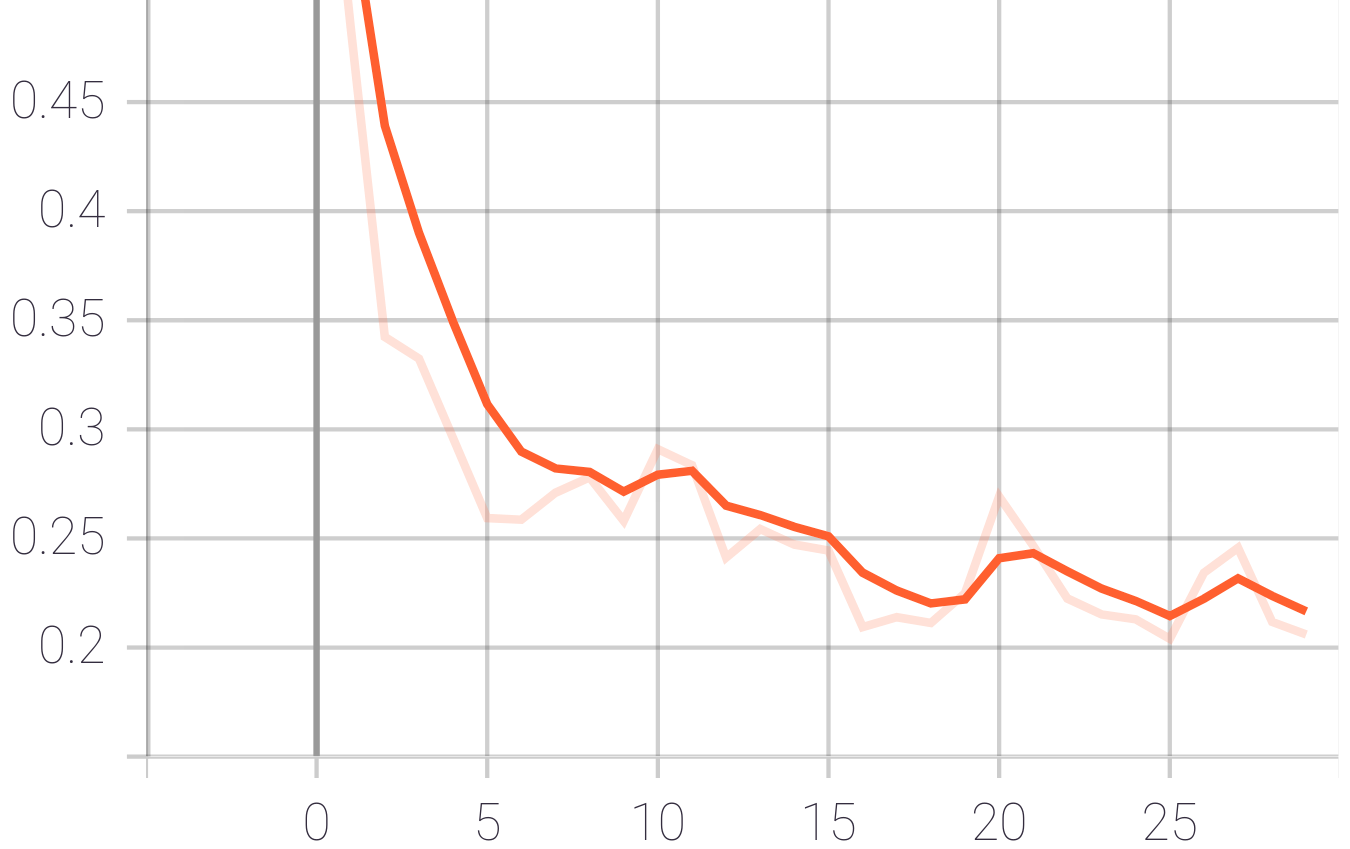
\includegraphics[width=0.45\textwidth]{./hinhanh/chap6/mask_loss_t10.png}}%
		\hfill % <-- Seperation
		\caption{Comparison between Test 3 and Test 10 training mask loss.}
		\label{fig:mask_loss_12}
	\end{figure}

	\textbf{Noted:} In training phrase, we did not pay much attention on training speed due to its similarity. However, the only thing that we can conclude from these tests is that the training speed of the test employing Resnet101 as backbone is a little longer than the one employing Resnet50 (around 60 minutes compared to around 70 minutes). Last but not least, the type of optimizer, learning rate, and weight decay also affect the training speed but not not worth considering.
	
\subsection{Inference}
\label{subsection:mrcnn_inference}
\noindent
	
	The testing phrase was executed on the PC with hardware as following:
	
	\begin{itemize}
		\item CPU Intel Core i5 8th.
		\item RAM 12GB.
	\end{itemize}
	
	Even with this minimum system, Mask R-CNN could generate mask with around 1~2 second for each testing image. The result was shown in Figure \ref{fig:train_test_result}.
	
	\begin{figure}[H]
		\centering
		\subcaptionbox{Generated mask on training sample.}{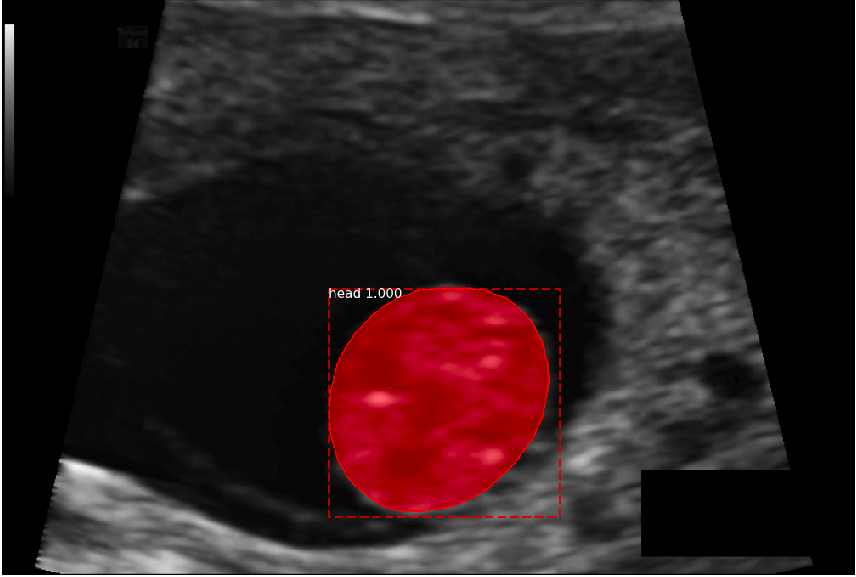
\includegraphics[width=0.45\textwidth]{./hinhanh/chap6/training_result.png}}%
		\hfill % <-- Seperation
		\subcaptionbox{Generated mask on testing sample.}{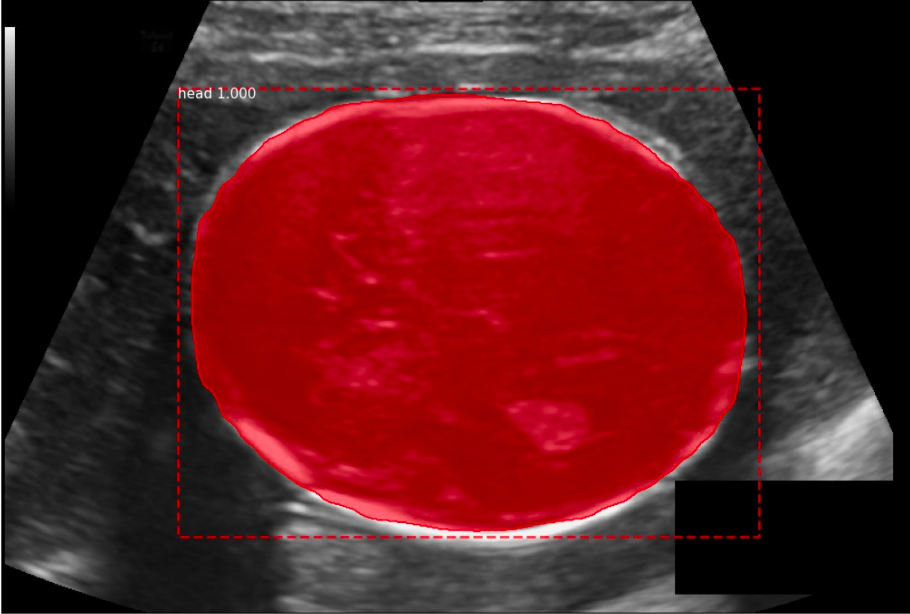
\includegraphics[width=0.45\textwidth]{./hinhanh/chap6/testing_result.png}}%
		\hfill % <-- Seperation
		\caption{We can see that segmentation part on testing sample were not perfect as training one. Therefore, the perimeter was estimated from this mask would be affected.}
		\label{fig:train_test_result}
	\end{figure}
	
	As we can see from Figure \ref{fig:train_test_result}, the generated mask was fit perfectly on the fetus' head. Yet, the model was not robust enough on the testing image (we can still see the white part of the skull that had not covered yet by the mask).
	
\section{Building the Restful API}
\noindent

	In this section, we will introduce our proposed system that includes five components includes 2 parts to transfer and manage the input, and 3 parts to process HC images and estimate the perimeter of the fetus' head. Each of the components is an restful API which works on specific task (inspired from micro service design). Therefore, in the future, we can easily scale up the number of workers (API) to speed up the process and manage them more conveniently in the deployment phrase. For more details, the system's design is shown in \ref{fig:hc_system}.
	
	\begin{figure}[H]
		\centering
		{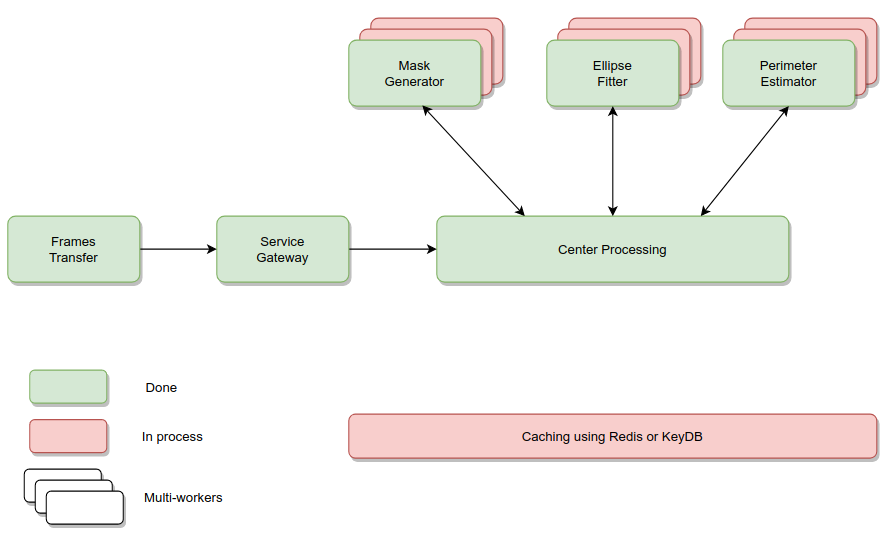
\includegraphics[width=0.9\textwidth]{./hinhanh/chap6/hc_system.png}}
		\caption{Proposed demo HC estimator system.}
		\label{fig:hc_system}
	\end{figure}

\subsection{Service Gateway}
\noindent

	Briefly, service gateway is an API that receives fetus' head from multiple sources such as images, video, or even streaming form. We decided to separate it to be standalone in order to process multiple transfer types more conveniently. However, in this thesis, this system is simply a demo so it only supports image transfer which is sent through a HTTP request.
	
	More precisely, the input data for Service Gateway are pixel size (to calculate the perimeter) and image of fetus' head in RGB color channel \ref{subsection:dataset}, .
	
\subsection{Center Processing}
\noindent

	This API, in short, it is like a CPU that sends data and receives result to/from others APIs. To be more specific:
	
	\begin{itemize}
		\item Firstly, it sends a image to Mask Generator, and then receive a binary mask.
		\item Secondly, it sends the binary mask and the image to Ellipse Fitter, and then receive an ellipse that fits on the mask.
		\item Finally, the ellipse's information is processed by Perimeter estimator to calculate the circumference of the ellipse (which is the fetus' head).
	\end{itemize}
	
	Besides, it works as a manager to monitor, report, etc.. the process of others APIs. Moreover, because we plan to increase the number of workers for specific task as in Figure \ref{fig:hc_system}, it is necessary to have a center processing to control the work flow of the system.

\subsection{Mask Generator}
\noindent
	
	As the first processing stage, Mask Generator receives a request from Center Processing to segment the fetus's head in an RGB image and returns a binary mask for it. Based on previous experiments, we decide to use the weights from \textit{Test 3} (which is our best model) to build Mask Generator API despite its imperfection in inference stage (but the result is still acceptable) as Figure \ref{fig:train_test_result} shows. 
	
	Even though the whole mask generating process is worked on a non-GPU computer, it still maintains the processing speed at 1 to 2s per image. Therefore, with a better hardware, we believe that the processing speed will definitely decrease and may achieve real-time processing speed to a certain extent.
	
\subsection{Ellipse Fitter}
\noindent

	After generating mask for the fetus' head, the Contour-finding and the Ellipse-specific algorithms are applied to adjust the polygon shape of the mask to the ellipse shape as in Figure \ref{fig:post_process}.
	
	\begin{figure}[H]
		\centering
		\subcaptionbox{The binary mask.}{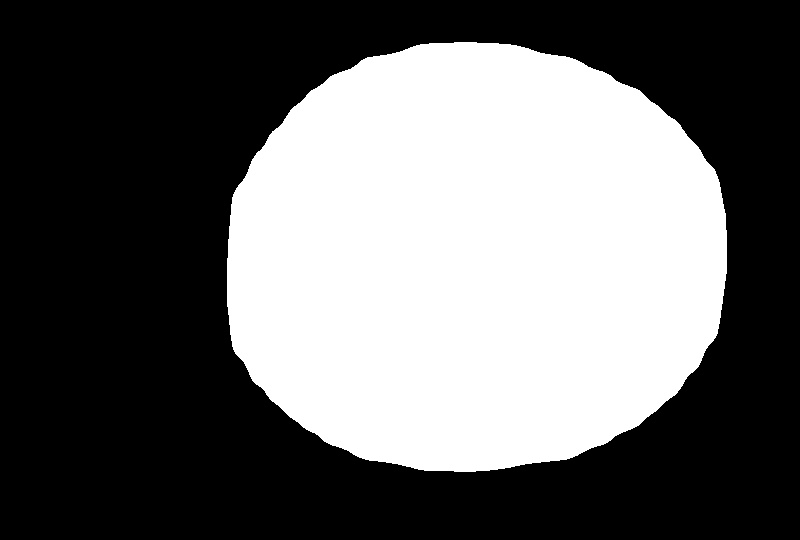
\includegraphics[width=0.45\textwidth]{./hinhanh/chap6/crop_mask.jpg}}%
		\hfill % <-- Seperation
		\subcaptionbox{The ellipse boundary on the fetus' head.}{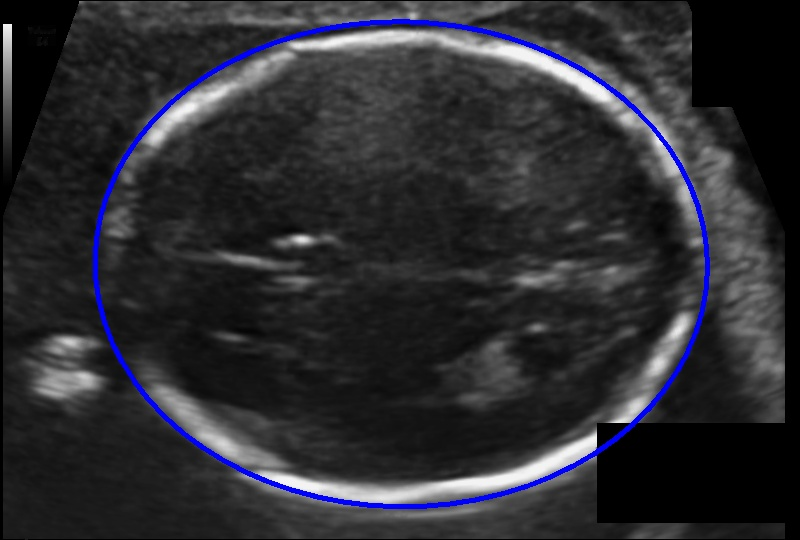
\includegraphics[width=0.45\textwidth]{./hinhanh/chap6/ellipse_on_crop_mask.jpg}}%
		\hfill % <-- Seperation
		\caption{Combine finding contour algorithm with ellipse fitting one to  it an ellipse on the image.}
		\label{fig:post_process}
	\end{figure}

	Precisely, a curve joining of all continuous points (along the boundary of the binary mask) is found by using algorithm from \cite{findContours}. Despite this method is simple to implement through OpenCV, it works quite efficiently on our binary mask.
	
	
	For an ellipse, its function requires a set $ \chi = (x^2, xy, y^2, x, y, 1)\ $. However, we only need five parameters to define an ellipse on 2D space. 
	
	\begin{itemize}
		\item (x, y): center x, center y.
		\item (MA, ma): semi axes a, semi axes b.
		\item Angle radian
	\end{itemize}
	
	To achieve this goal, we fit the ellipse around this set of 2D points by employing the Direct Least Square approach from \cite{direct_ellipse}.
	
\subsection{Perimeter Estimator}
\noindent
	
	After receiving the ellipse's coordinates from Ellipse Fitter API, we estimate the ellipse's perimeter by employing Ramanujan’s formula \cite{perimeter}. The approximation of Ramanujan is demonstrated as in Equation \eqref{eq:perimeter}:
	
	\[ h = \frac{(a-b)^2}{(a+b)^2} \]
	
	\[ p \approx \pi (a+b) (1 + \frac{3h}{(10 + \sqrt{4 - 3h})} ) \label{eq:perimeter} \]

\noindent
	Then we multiply the $p$ with the pixel size to scale the result to the exact measure.
	
\subsection{Result}
\noindent

	To evaluation the whole system, we tested it with 335 ultrasound images and then we submitted the result to  \href{https://hc18.grand-challenge.org/}{Grand Challenge}. As the result, we were ranked at 1077 position with several metrics.
	
	\textbf{Metrics to evaluate the system:}
	\begin{itemize}
		\item "DICE": Also called F1 score, it is 2 * the Area of Overlap divided by the total number of pixels in both images (it is similar to IoU).
		\item "Difference": Similar to loss function, it is described as $x - y$.
		\item "Absolute Difference": It is difference metric but in absolute value.
		\item "Hausdorff Distance": Calculate the distance between 2 subsets of a metric space are from each other.
	\end{itemize}
%
%	\textbf{Difference:}
%	\begin{itemize}
%		\item "max": 27.589732124216823,
%		\item "min": -0.6480596018764686,
%		\item "std": 4.33538798698353,
%		\item "25pc": 4.394918205609386,
%		\item "50pc": 6.114941307429092,
%		\item "75pc": 8.74297314561646,
%		\item "mean": 7.147501055171521,
%		\item "count": 335.0
%	\end{itemize}
%	
%	\textbf{DICE trimester 1:}
%	\begin{itemize}
%		\item "max": 97.13935203256567,
%		\item "min": 76.75946495249799,
%		\item "std": 4.762801395468964,
%		\item "25pc": 85.62838488544139,
%		\item "50pc": 88.8016218891177,
%		\item "75pc": 92.7723271301243,
%		\item "mean": 88.74547608698568,
%		\item "count": 55.0
%	\end{itemize}
%
%	\textbf{DICE trimester 2:}
%	\begin{itemize}
%		\item "max": 97.0691841623221,
%		\item "min": 77.47039916485811,
%		\item "std": 3.3353566574286297,
%		\item "25pc": 83.26670659930204,
%		\item "50pc": 85.55823051459525,
%		\item "75pc": 87.29931334288395,
%		\item "mean": 85.63891977747174,
%		\item "count": 233.0
%	\end{itemize}
%
%	\textbf{DICE trimester 3:}
%	\begin{itemize}
%		\item "max": 90.40598274885838,
%		\item "min": 78.04261888610793,
%		\item "std": 3.298341158642274,
%		\item "25pc": 83.15553019467893,
%		\item "50pc": 85.53754670022215,
%		\item "75pc": 87.85791957902292,
%		\item "mean": 85.23085976507201,
%		\item "count": 47.0
%	\end{itemize}
%
%	\textbf{Hausdorff distance:}
%	\begin{itemize}
%		\item "max": 20.589144777463485,
%		\item "min": 0.7724761587361798,
%		\item "std": 3.583340499351782,
%		\item "25pc": 5.516364786956328,
%		\item "50pc": 7.548516888575833,
%		\item "75pc": 9.419397962500073,
%		\item "mean": 7.581017919690942,
%		\item "count": 335.0
%	\end{itemize}
%
%	\textbf{Absolute difference:}
%	\begin{itemize}
%		\item "max": 27.589732124216823,
%		\item "min": 0.6480596018764686,
%		\item "std": 4.3289838125839815,
%		\item "25pc": 4.394918205609386,
%		\item "50pc": 6.114941307429092,
%		\item "75pc": 8.74297314561646,
%		\item "mean": 7.151370067720037,
%		\item "count": 335.0
%	\end{itemize}
%
%	\textbf{Difference trimester 1:}
%	\begin{itemize}
%		\item "max": 15.111908868158608,
%		\item "min": 1.2812882510039572,
%		\item "std": 2.9241650358535636,
%		\item "25pc": 3.134473332958102,
%		\item "50pc": 4.602075402152096,
%		\item "75pc": 6.087198198104765,
%		\item "mean": 5.135097830934518,
%		\item "count": 55.0
%	\end{itemize}
%
%	\textbf{Difference trimester 2:}
%	\begin{itemize}
%		\item "max": 24.749099690650667,
%		\item "min": -0.6480596018764686,
%		\item "std": 3.579054028927821,
%		\item "25pc": 4.464146812138978,
%		\item "50pc": 6.026485291046242,
%		\item "75pc": 7.730095196420621,
%		\item "mean": 6.635340857744364,
%		\item "count": 233.0
%	\end{itemize}
%
%	\textbf{Difference trimester 3:}
%	\begin{itemize}
%		\item "max": 27.589732124216823,
%		\item "min": 0.6867050791128122,
%		\item "std": 5.584556464260941,
%		\item "25pc": 9.190157286174411,
%		\item "50pc": 11.662282500140009,
%		\item "75pc": 14.501014051515938,
%		\item "mean": 12.041447934609026,
%		\item "count": 47.0
%	\end{itemize}
%
%	\textbf{Hausdorff distance trimester 1:}
%	\begin{itemize}
%		\item "max": 6.097752780066,
%		\item "min": 0.7724761587361798,
%		\item "std": 1.1635430749332072,
%		\item "25pc": 1.98026176953945,
%		\item "50pc": 2.7580496387675,
%		\item "75pc": 3.6799445304227216,
%		\item "mean": 2.8235145949238367,
%		\item "count": 55.0
%	\end{itemize}
%
%	\textbf{Hausdorff distance trimester 2:}
%	\begin{itemize}
%		\item "max": 14.658116046154605,
%		\item "min": 1.0214043471768,
%		\item "std": 2.045828977818262,
%		\item "25pc": 6.316217417726442,
%		\item "50pc": 7.616355581727,
%		\item "75pc": 8.87503939518,
%		\item "mean": 7.535175687838671,
%		\item "count": 233.0
%	\end{itemize}
%
%	\textbf{Hausdorff distance trimester 3:}
%	\begin{itemize}
%		\item "max": 20.589144777463485,
%		\item "min": 8.011363070117723,
%		\item "std": 3.0255606034609572,
%		\item "25pc": 11.575047545355172,
%		\item "50pc": 12.37692592766892,
%		\item "75pc": 15.573101160804221,
%		\item "mean": 13.37556947040946,
%		\item "count": 47.0
%	\end{itemize}
%
%	\textbf{Absolute difference trimester 1:}
%	\begin{itemize}
%		\item "max": 15.111908868158608,
%		\item "min": 1.2812882510039572,
%		\item "std": 2.9241650358535636,
%		\item "25pc": 3.134473332958102,
%		\item "50pc": 4.602075402152096,
%		\item "75pc": 6.087198198104765,
%		\item "mean": 5.135097830934518,
%		\item "count": 55.0
%	\end{itemize}
%
%	\textbf{Absolute difference trimester 2:}
%	\begin{itemize}
%		\item "max": 24.749099690650667,
%		\item "min": 0.6480596018764686,
%		\item "std": 3.5686772160242395,
%		\item "25pc": 4.464146812138978,
%		\item "50pc": 6.026485291046242,
%		\item "75pc": 7.730095196420621,
%		\item "mean": 6.64090360110811,
%		\item "count": 233.0
%	\end{itemize}
%
%	\textbf{Absolute difference trimester 3:}
%	\begin{itemize}
%		\item "max": 27.589732124216823,
%		\item "min": 0.6867050791128122,
%		\item "std": 5.584556464260941,
%		\item "25pc": 9.190157286174411,
%		\item "50pc": 11.662282500140009,
%		\item "75pc": 14.501014051515938,
%		\item "mean": 12.041447934609026,
%		\item "count": 47.0
%	\end{itemize}



\begin{longtable}[c]{|p{0.08\textwidth}|p{0.22\textwidth}|p{0.22\textwidth}|p{0.22\textwidth}|p{0.22\textwidth}|}
	\hline
	& \multicolumn{1}{c|}{\textbf{DICE}} & \multicolumn{1}{c|}{\textbf{DICE T1}} & \multicolumn{1}{c|}{\textbf{DICE T2}} & \multicolumn{1}{c|}{\textbf{DICE T3}} \\ \hline
	\endhead
	\textbf{Max} & 27.589732124216823 & 27.589732124216823 & 97.0691841623221 & 90.40598274885838 \\ \hline
	\textbf{Min} & 76.75946495249799 & 76.75946495249799 & 77.47039916485811 & 78.04261888610793 \\ \hline
	\textbf{Std} & 3.7815463871178943 & 4.762801395468964 & 3.3353566574286297 & 3.298341158642274 \\ \hline
	\textbf{25pc} & 83.50825381011883 & 85.62838488544139 & 83.26670659930204 & 83.15553019467893 \\ \hline
	\textbf{50pc} & 85.81469956490609 & 88.8016218891177 & 85.55823051459525 & 85.53754670022215 \\ \hline
	\textbf{75pc} & 88.01129094018415 & 92.7723271301243 & 87.29931334288395 & 87.85791957902292 \\ \hline
	\textbf{Mean} & 86.09170119968213 & 88.74547608698568 & 85.63891977747174 & 85.23085976507201 \\ \hline
	\textbf{Count} & 335 & 55 & 233 & 47 \\ \hline
	
	
	\caption{DICE metrics}
	\label{table:dice}
\end{longtable}


\begin{longtable}[c]{|p{0.08\textwidth}|p{0.22\textwidth}|p{0.22\textwidth}|p{0.22\textwidth}|p{0.22\textwidth}|}
	\hline
	& \multicolumn{1}{c|}{\textbf{Difference}} & \multicolumn{1}{c|}{\textbf{Difference T1}} & \multicolumn{1}{c|}{\textbf{Difference T2}} & \multicolumn{1}{c|}{\textbf{Difference T3}} \\ \hline
	\endhead
	\textbf{Max} & 27.589732124216823 & 15.111908868158608 & 24.749099690650667 & 27.589732124216823 \\ \hline
	\textbf{Min} & -0.64805960187646 & 1.2812882510039572 & -0.64805960187646 & 0.6867050791128122 \\ \hline
	\textbf{Std} & 4.33538798698353 & 2.9241650358535636 & 3.579054028927821 & 5.584556464260941 \\ \hline
	\textbf{25pc} & 4.394918205609386 & 3.134473332958102 & 4.464146812138978 & 9.190157286174411 \\ \hline
	\textbf{50pc} & 6.114941307429092 & 4.602075402152096 & 6.026485291046242 & 11.662282500140009 \\ \hline
	\textbf{75pc} & 8.74297314561646 & 6.087198198104765 & 7.730095196420621 & 14.501014051515938 \\ \hline
	\textbf{Mean} & 7.147501055171521 & 5.135097830934518 & 6.635340857744364 & 12.041447934609026 \\ \hline
	\textbf{Count} & 355 & 55 & 233 & 47 \\ \hline
	
	
	\caption{Difference metrics}
	\label{table:difference}
\end{longtable}

\begin{longtable}[c]{|p{0.08\textwidth}|p{0.22\textwidth}|p{0.22\textwidth}|p{0.22\textwidth}|p{0.22\textwidth}|}
	\hline
	& \multicolumn{1}{c|}{\textbf{Abs diff}} & \multicolumn{1}{c|}{\textbf{Abs diff T1}} & \multicolumn{1}{c|}{\textbf{Abs diff T2}} & \multicolumn{1}{c|}{\textbf{Abs diff T3}} \\ \hline
	\endhead
	\textbf{Max} & 27.589732124216823 & 15.111908868158608 & 24.749099690650667 & 27.589732124216823 \\ \hline
	\textbf{Min} & 0.6480596018764686 & 1.2812882510039572 & 0.6480596018764686 & 0.6867050791128122 \\ \hline
	\textbf{Std} & 4.3289838125839815 & 2.9241650358535636 & 3.5686772160242395 & 5.584556464260941 \\ \hline
	\textbf{25pc} & 4.394918205609386 & 3.134473332958102 & 4.464146812138978 & 9.190157286174411 \\ \hline
	\textbf{50pc} & 6.114941307429092 & 4.602075402152096 & 6.026485291046242 & 11.662282500140009 \\ \hline
	\textbf{75pc} & 8.74297314561646 & 6.087198198104765 & 7.730095196420621 & 14.501014051515938 \\ \hline
	\textbf{Mean} & 7.151370067720037 & 5.135097830934518 & 6.64090360110811 & 12.041447934609026 \\ \hline
	\textbf{Count} & 355 & 55 & 233 & 47 \\ \hline
	
	
	\caption{Absolute difference metrics}
	\label{table:abs_diff}
\end{longtable}

\begin{longtable}[c]{|p{0.08\textwidth}|p{0.22\textwidth}|p{0.22\textwidth}|p{0.22\textwidth}|p{0.22\textwidth}|}
	\hline
	& \multicolumn{1}{c|}{\textbf{Hausdorff dis}} & \multicolumn{1}{c|}{\textbf{Hausdorff dis T1}} & \multicolumn{1}{c|}{\textbf{Hausdorff dis T2}} & \multicolumn{1}{c|}{\textbf{Hausdorff dis T3}} \\ \hline
	\endhead
	\textbf{Max} & 20.589144777463485 & 6.097752780066 & 14.658116046154605 & 20.589144777463485 \\ \hline
	\textbf{Min} & 0.7724761587361798 & 0.7724761587361798 & 1.0214043471768 & 8.011363070117723 \\ \hline
	\textbf{Std} & 3.583340499351782 & 1.1635430749332072 & 2.045828977818262 & 3.0255606034609572 \\ \hline
	\textbf{25pc} & 5.516364786956328 & 1.98026176953945 & 6.316217417726442 & 11.575047545355172 \\ \hline
	\textbf{50pc} & 7.548516888575833 & 2.7580496387675 & 7.616355581727 & 12.37692592766892 \\ \hline
	\textbf{75pc} & 9.419397962500073 & 3.6799445304227216 & 8.87503939518 & 15.573101160804221 \\ \hline
	\textbf{Mean} & 7.581017919690942 & 2.8235145949238367 & 7.535175687838671 & 13.37556947040946 \\ \hline
	\textbf{Count} & 355 & 55 & 233 & 47 \\ \hline
	
	
	\caption{Difference metrics}
	\label{table:difference}
\end{longtable}
	